\section{Problem}\label{problem}

Density functional theory (DFT) offers computationally affordable way of
describing static and dynamic properties of superfluid He. In general,
the DFT models yield single particle-like Schrödinger equations with a
nonlinear potential term that accounts for all the many-body
interactions. The resulting equations can be analytically solved for
small amplitude plane wave excitations in the bulk whereas fully
numerical solution must be sought in more complicated cases. Here we
discuss a numerical method that can be used in solving the
time-dependent nonlinear Schrödinger equation in both real and imaginary
times.\footnote{Lehtovaara, Lauri, Toni Kiljunen, and Jussi Eloranta.
  ``Efficient numerical method for simulating static and dynamic
  properties of superfluid helium.'' Journal of Computational Physics
  194.1 (2004): 78-91.}

\section{The Imaginary Time Propagation
Method}\label{the-imaginary-time-propagation-method}

The imaginary time propagation method (ITP) relies on solving the
time-dependent Schrödinger equation

\begin{equation}
\label{eq:timedepSch}
i\hbar\frac{\partial \psi(r,t)}{\partial t}= \hat{H}\psi(r,t)
\end{equation}

in imaginary time. We perform a Wick Rotation (setting \(t=-i\tau\)) to
transform eq. \ref{eq:timedepSch} into a simple diffusion equation

\begin{equation}
\label{eq:itpSch}
\frac{\partial \psi(r,\tau)}{\partial
\tau}=-\frac{\hat{H}}{\hbar}\psi(r,\tau)
\end{equation}

\subsection{Solution to the Diffusion
Equation}\label{solution-to-the-diffusion-equation}

The formal solution to eqn. eq. \ref{eq:itpSch} is given by

\begin{equation}
\psi(r,\tau)=\exp(-\hat{H}\tau/\hbar)\psi(r,0)
\end{equation}

Which can be thought of as the analog to an power solution or subspace
iteration. As \(\tau\to\infty\), \(\psi(r,\tau)\) becomes proportional
to \(\phi_0(r)\). In other words, iterated \(\psi\) functions will
converge on the eigenfunction for the base state of the time-equation
(eq. \ref{eq:timedepSch}).

In practice, a random vector is chosen as the initial state. A
time-propagation will yield the ground state eigenvector. If a vector
other than the ground state is desired, \(N\) separate wave functions
are propagated. Each higher state eigenvector is required to be
orthogonal to the lower eigenvectors and are thus discovered through the
iterative process. Approximate orthogonality is enforced in the
following way.

\begin{equation}
\label{eq:appxOrth}
\pdif{\psi_i(r,\tau)}{\tau} = -\frac{\hat{H}}{\hbar}\psi(r,\tau)-\lambda\sum_{j < i}^N |\langle \psi_j(r,\tau)|\psi_i(r,\tau)\rangle|^2
\end{equation}

In order to implement the solution computationally, the exponential
operator is approximated using the Cayley unitary form:

\begin{equation}
\label{eq:CayleyExpansion}
\exp(-H\Delta\tau)\approx\biggP{1+\frac{1}{2}H\Delta\tau}^{-1}\biggP{1-\frac{1}{2}H\Delta\tau}
\end{equation}

Which turns the eigenvalue problem into a linear problem.

\begin{equation}
\label{eq:LinearCayleyExpansion}
\biggP{1+\frac{1}{2}H\Delta\tau}\psi(r,\tau+\Delta\tau)=\biggP{1-\frac{1}{2}H\Delta\tau}\psi(r,\tau)
\end{equation}

\begin{description}
\itemsep1pt\parskip0pt\parsep0pt
\item[Stopping Criteria]
A formula for the absolute error, \(\Delta E_i\) present in
\(E_i(\tau)\) can be written in terms of the quantum mechanical standard
deviation of \(H\) as follows:
\end{description}

\begin{equation}
\label{eq:error}
\Delta E_i = |E_i -\langle\psi_i(r,\tau)|H|\psi_i(r,\tau)|\leq\sqrt{2}\sqrt{\langle\psi_i(r,\tau)|H^2|\psi_i(r,\tau)\rangle-\langle\psi_i(r,\tau)|H|\psi_i(r,\tau)\rangle^2}
\end{equation}

and is used as a stopping criteria.

\pagebreak

\section{Application}\label{application}

ITP has been applied in the following manner:

\begin{quote}
Helium clusters were modeled by the Orsay-Trento DFT (OT-DFT) and the
interaction with the guest molecule was included through an external
potential. To compute the effective moment of inertia of the
molecule--helium complex, we include an additional energy term of the
form \(-\omega L_z\) and compute the ``rotating'' groundstate energy by
minimizing
\end{quote}

\begin{equation}
\label{eq:OTDFT}
E[\Psi,\omega]=\int\biggBc{\frac{\hbar^2}{2m}|\nabla\Psi|^2+\epsilon_{OT}[\Psi]+V_{X-\text{He}}|\Psi|^2-\omega \Psi*L_z\Psi}
\end{equation}

\begin{quote}
with respect to the liquid helium complex order parameter \(\Psi\)
(``effective wavefunction'') normalized to the number of particles
\(N\), where \(m\) is the helium atom mass, \(\epsilon_{OT}\) represent
the Orsay-Trento energy density functional, \(V_{X-\text{He}}\) is the
molecule-helium interaction (molecule oriented along the \(x\)-axis),
\(\omega\) is a fixed parameter representing the rotation frequency, and
\(L_z\) is the angular momentum operator along the \(z\) axis going
through a given point \(\vec{r}_0\).\footnote{Mateo, David, Frisly
  Gonzalez, and Jussi Eloranta. ``Rotational Superfluidity in Small
  Helium Droplets.'' The Journal of Physical Chemistry A (2014).}
\end{quote}

\subsection{Computational Solution}\label{computational-solution}

The non-linear Schrödinger-type equation arising from the minimization
of eq. \ref{eq:OTDFT} is solved by means of imaginary time propagation.

Liquid He can be described using DFT, by reducing the many-body problem
to an effective single particle Schrödinger-like equation.\footnote{Lehtovaara,
  Lauri, Toni Kiljunen, and Jussi Eloranta. ``Efficient numerical method
  for simulating static and dynamic properties of superfluid helium.''
  Journal of Computational Physics 194.1 (2004): 78-91.}

\begin{equation}
\label{eq:OTDFTtoSch}
i\hbar\pdif{\Psi}{t}=\pdif{E}{\psi*}\Psi
\end{equation}

an equation of the form of eqn \ref{eq:timedepSch} for
\(H=\pdif{E}{\psi*}\). We then using the ITP method to numerically solve
this equation.

\subsection{Finding the Ground State}\label{finding-the-ground-state}

\begin{verbatim}

import numpy as np
import numpy.linalg as la
import math, time
import matplotlib.pyplot as plt
from sys import argv
import datetime
%matplotlib inline


k = 100

eps = 10E-6
times = np.array([[0.,0.]]) 
temp_times = times
H = np.random.rand(k+200,k+200)
H = H.T.dot(H)
file = datetime.datetime.now().strftime("%Y%m%d%H%M%S")

for i in range(k):
        # print i
        i = i+1
        n = i
        err = 1
        int_H = H[0:n,0:n]
        iterations = 0
        start = time.clock()

        phi0 = np.random.rand(n)
        # print la.eig(H)[1].T
        CayleyN = (np.identity(n)-0.5*int_H)
        CayleyP = (np.identity(n)+0.5*int_H)

        while(err > eps):
                iterations += 1
                phi1 = la.solve(CayleyP,CayleyN.dot(phi0))
                mu = math.sqrt(phi1.dot(phi1))
                phi1 = phi1/mu  
                err = math.sqrt(2)*math.sqrt(abs(phi1.dot(int_H.dot(int_H)).dot(phi1)- (phi1.dot(int_H).dot(phi1))**2))
                phi0 = phi1

        end = time.clock()
        delta_t = end-start
        temp_times[0][0] = i
        temp_times[0][1] = delta_t
        times = np.concatenate((times,temp_times),axis=0)
        np.savetxt(file,times,fmt='%.4e')

        
plt.plot(times[:k,0],times[:k,1])

plt.show()
\end{verbatim}

\begin{figure}[htbp]
\centering
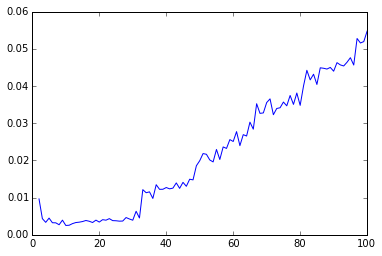
\includegraphics{ExcitedStates_files/ExcitedStates_9_0.png}
\caption{Times \(n=100\)}
\end{figure}

\pagebreak

\subsubsection{Ground State eigenvector found using ITP
Method}\label{ground-state-eigenvector-found-using-itp-method}

\begin{verbatim}
array([ 0.095811,  0.103336,  0.101997,  0.103104,  0.09915 ,  0.104293,
        0.097661,  0.098985,  0.099519,  0.103466,  0.096878,  0.098705,
        0.0966  ,  0.099749,  0.103957,  0.097404,  0.096983,  0.099913,
        0.095697,  0.09801 ,  0.102899,  0.096146,  0.099466,  0.097908,
        0.103759,  0.098855,  0.103091,  0.098825,  0.101815,  0.099494,
        0.096614,  0.100962,  0.095844,  0.103862,  0.100759,  0.099581,
        0.098617,  0.106259,  0.097449,  0.102104,  0.097868,  0.102439,
        0.096882,  0.100899,  0.092935,  0.101082,  0.10574 ,  0.1009  ,
        0.099533,  0.101069,  0.106548,  0.102221,  0.096897,  0.097431,
        0.095495,  0.094038,  0.101569,  0.097085,  0.095079,  0.102557,
        0.106596,  0.099939,  0.100268,  0.103684,  0.097932,  0.097291,
        0.096313,  0.098528,  0.091565,  0.103261,  0.102006,  0.101996,
        0.103406,  0.094932,  0.097117,  0.10008 ,  0.100454,  0.095418,
        0.102195,  0.100689,  0.105295,  0.100508,  0.094709,  0.096054,
        0.103639,  0.101266,  0.095723,  0.101786,  0.101302,  0.100328,
        0.106601,  0.09259 ,  0.104864,  0.105139,  0.101007,  0.100833,
        0.100051,  0.100539,  0.107391,  0.097154])
\end{verbatim}

\subsubsection{Ground State eigenvector found using
Numpy}\label{ground-state-eigenvector-found-using-numpy}

Found using \texttt{numpy.linalg.eig()} which is a python implementation
of \texttt{\_geev} included with \texttt{LAPACK}.

\begin{verbatim}
la.eig(int_H)[1][:,0]

array([ 0.095811,  0.103336,  0.101997,  0.103104,  0.09915 ,  0.104293,
        0.097661,  0.098985,  0.099519,  0.103466,  0.096878,  0.098705,
        0.0966  ,  0.099749,  0.103957,  0.097404,  0.096983,  0.099913,
        0.095697,  0.09801 ,  0.102899,  0.096146,  0.099466,  0.097908,
        0.103759,  0.098855,  0.103091,  0.098825,  0.101815,  0.099494,
        0.096614,  0.100962,  0.095844,  0.103862,  0.100759,  0.099581,
        0.098617,  0.106259,  0.097449,  0.102104,  0.097868,  0.102439,
        0.096882,  0.100899,  0.092935,  0.101082,  0.10574 ,  0.1009  ,
        0.099533,  0.101069,  0.106548,  0.102221,  0.096897,  0.097431,
        0.095495,  0.094038,  0.101569,  0.097085,  0.095079,  0.102557,
        0.106596,  0.099939,  0.100268,  0.103684,  0.097932,  0.097291,
        0.096313,  0.098528,  0.091565,  0.103261,  0.102006,  0.101996,
        0.103406,  0.094932,  0.097117,  0.10008 ,  0.100454,  0.095418,
        0.102195,  0.100689,  0.105295,  0.100508,  0.094709,  0.096054,
        0.103639,  0.101266,  0.095723,  0.101786,  0.101302,  0.100328,
        0.106601,  0.09259 ,  0.104864,  0.105139,  0.101007,  0.100833,
        0.100051,  0.100539,  0.107391,  0.097154])
\end{verbatim}

\pagebreak

\subsubsection{Error between the two
vectors}\label{error-between-the-two-vectors}

\begin{verbatim}
abs(la.eig(int_H)[1][:,0])-abs(phi0)

array([ -1.804403e-10,   1.524185e-09,  -1.381993e-10,   9.191934e-10,
         1.477085e-09,   1.270410e-09,  -1.272802e-09,  -1.037408e-09,
        -1.273373e-10,  -5.737870e-10,  -1.685339e-09,  -2.375439e-10,
        -9.888992e-10,   1.954964e-09,   2.007974e-09,  -1.507765e-09,
         8.474579e-10,  -1.961359e-09,  -8.043330e-10,  -2.187794e-09,
        -2.569797e-09,  -1.019212e-10,  -1.232498e-09,  -1.745826e-09,
         4.522222e-10,   7.244396e-10,   4.752562e-10,  -9.960150e-10,
         1.370411e-09,  -1.203053e-10,  -2.146047e-09,   2.739398e-11,
         6.394539e-10,  -1.213031e-09,  -1.720872e-10,  -2.796302e-10,
        -4.815309e-11,   8.015536e-10,  -1.783063e-10,  -2.501262e-10,
         1.610441e-09,   8.197204e-10,   1.175502e-09,  -1.101852e-09,
        -6.593943e-10,   1.457115e-09,   1.568503e-10,  -3.935539e-10,
         6.345335e-11,  -2.458059e-10,   4.386881e-10,  -4.559281e-10,
        -7.530098e-10,  -1.158156e-09,  -5.343609e-11,  -7.870312e-10,
         2.439480e-10,  -1.675589e-10,   4.694113e-11,  -1.215481e-10,
         1.642119e-09,   1.536224e-10,   1.021933e-09,  -7.859301e-10,
         8.376032e-10,   3.359412e-10,  -1.024301e-09,  -8.439009e-10,
         7.276948e-10,  -4.532696e-10,   1.703726e-09,  -2.959827e-09,
        -2.067084e-10,  -1.355851e-09,  -5.654463e-10,   6.019744e-11,
        -3.579826e-10,  -2.465226e-09,  -6.073011e-10,   2.398757e-09,
        -4.412440e-10,  -3.493164e-10,  -4.600466e-11,   2.694824e-10,
         2.133818e-09,  -1.531635e-10,   1.728650e-09,   2.863394e-10,
         1.576883e-09,  -1.678248e-10,   4.619403e-10,   7.667073e-10,
         1.211877e-09,  -8.348254e-10,   6.230160e-10,   3.981608e-10,
         1.033806e-09,   7.384125e-10,   6.549274e-10,   1.176959e-09])
\end{verbatim}

\subsection{How many Iterations?}\label{how-many-iterations}

\subsubsection{Finding an Excited
Eigenstate}\label{finding-an-excited-eigenstate}

Given our basic
